\graphicspath{{/Users/emiliendurif/Documents/prepa/sujets/TP_sujets/TP_simulation/drone_d2C/}}

\subsection{Drone D2C}
\subsubsection{Pr�sentation}

Le Drone D2C est une maquette de drone quadricopt�re permettant de simuler les mouvement de tangage seul et d'en �tudier les diff�rentes performances.

On s'int�resse ici uniquement � l'asservissement autour de l'axe de tangage.


\begin{figure}[!htb]
\begin{tabular}{cc}
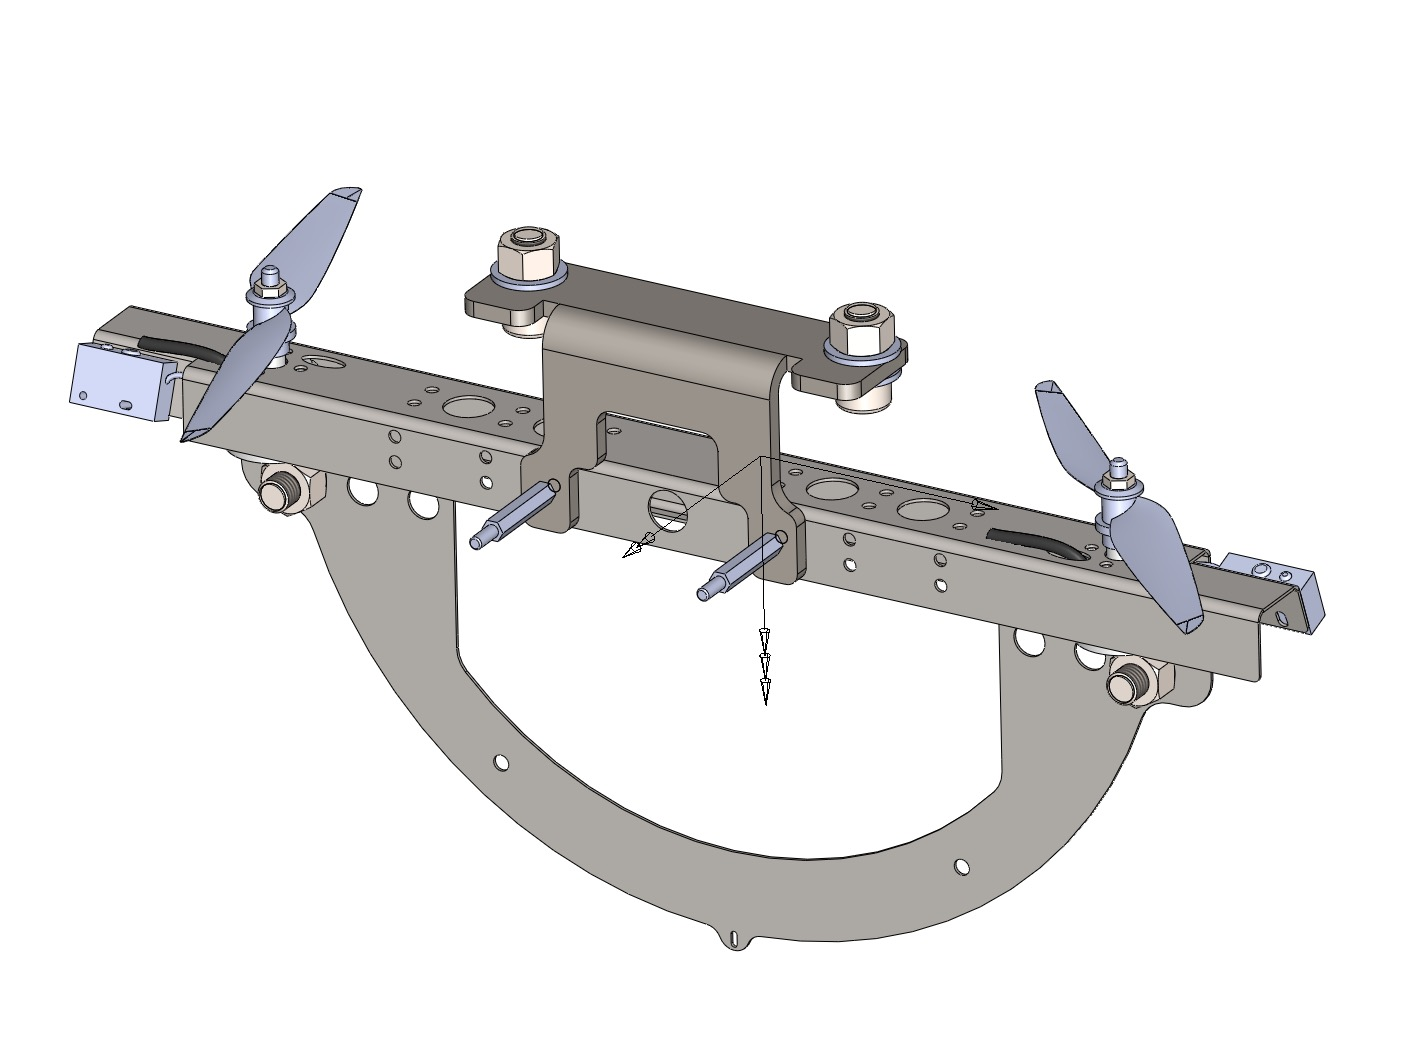
\includegraphics[width=0.7\textwidth]{images/drone_cao}
&
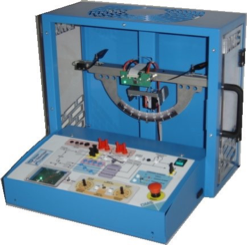
\includegraphics[width=0.3\textwidth]{images/drone_maquette}
\\
\end{tabular}
\end{figure}



\subsubsection{Analyse structurelle du drone D2C}

\question{Compl�ter la chaine fonctionnelle d�crivant la chaine cin�matique du drone D2C � l'aide de la documentation technique fourni sur le serveur.}

\begin{center}
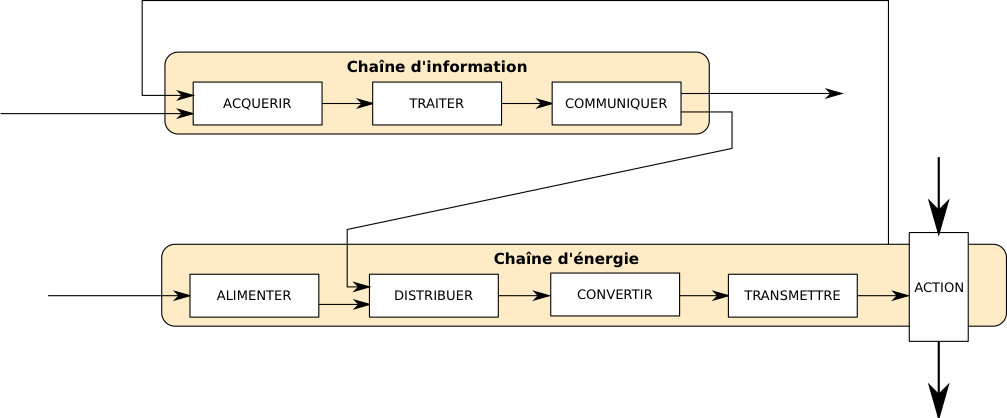
\includegraphics[width=1.0\textwidth]{images/chaine_fonctionnelle.png}
\end{center}



\subsubsection{Analyse du mod�le Simmechanics}

\question{
\begin{enumerate}
\item Copier le dossier "modele$\_$acausal" sur votre espace perso.
\item Placer le chemin d'acc�s de ce dossier dans la barre d'adresse Matlab.
\item Lancer Simulink et ouvrir le fichier d2C$\_$simmechanics.slx.
\item Ex�cuter le programme et observer le r�sultat de la simulation. 
\end{enumerate}
}


\question{A l'aide du mod�le Simmechanics, construire le graphe de liaison du syst�me et v�rifier sur le syst�me r�el sa coh�rence.}

\subsubsection{Prise en compte des effets a�rodynamiques}

\begin{figure}[!htb]
\begin{minipage}{0.5\textwidth}
On donne sur la courbe ci-contre la relation caract�risant une h�lice d'un point de vue a�rodynamique. On trace alors l'effort de portance en fonction de la vitesse de rotation de l'h�lice.
\end{minipage}
\begin{minipage}{0.5\textwidth}
\begin{center}
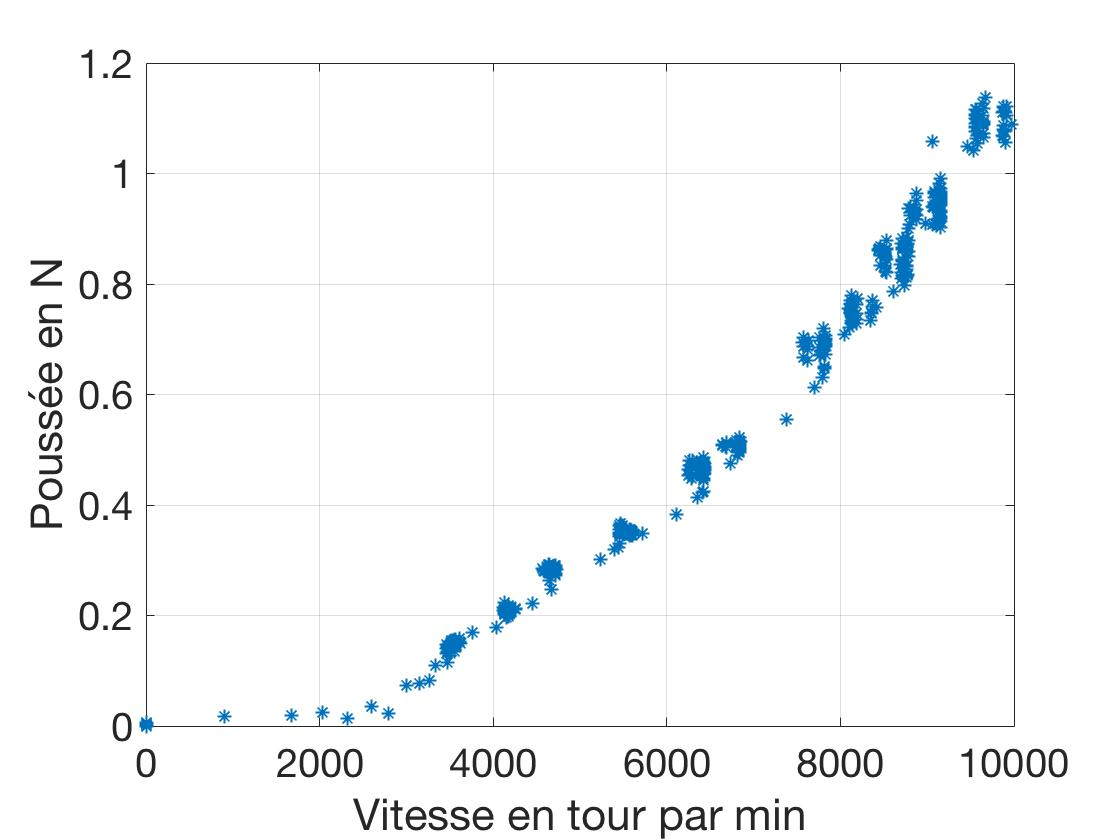
\includegraphics[width=1.0\textwidth]{images/Fp_Ne.jpg}
\end{center}
\end{minipage}
\end{figure}

\FloatBarrier
\question{Proposer un mod�le de comportement permettant de relier l'effort de portance (Pouss�e) en fonction de la vitesse de rotation des h�lices.}

\subsubsection{Mod�lisation de l'asservissement du syst�me}

\question{Ouvrir le fichier D2C$\_$boucle$\_$vitesse$\_$modelisation.slx et analyser l'asservissement en vitesse.}

\question{Proposer une m�thode pour impl�menter le mod�le Simmechanics dans ce mod�le.}

\question{A l'aide de la fichier 8 de la documentation technique du syst�me drone D2C, proposer une m�thode exp�rimentale pour identifier les constantes des blocs correspondant aux deux motorisations.}

\question{Mettre en oeuvre ces exp�rimentation et identifier les blocs correspondants.}

\question{Mettre en oeuvre la simulation et conclure.}


